\subsection{Risk on a Compatible Multiscale Family}\label{sec:geometry-experiment}
The first study evaluates the common null/spike family used in the lower-bound proof. At endpoint $T\in\{1024,4096,16384,65536\}$, batch $j$ has $2\cdot4^j$ competitors and lifetime $T/4^j$, for $j=0,\ldots,L-1$. We use $L\le3$ at the two smaller endpoints and $L\le4$ at the two larger ones. All groups survive the compatibility selection and contribute equally to the spectrum: $\cS_T=L\sqrt{2T}$ and $D_T^{\mathrm{eff}}=L$.

Each group has one reference arm. With probability $1/2$ all its candidates are below the reference; otherwise one uniformly selected candidate is above it. Independent configurations and deterministic increments in the reference means give one compatible stationary environment per replication. We use the proof's gap constant and the prespecified multipliers $a=4,8$, with $a=4$ in the main comparison. Larger multipliers preserve a legal prior but need not preserve the proof's total-variation bound. Each cell averages 128 independent draws of the environment and its Bernoulli observations. These finite-prior risks do not estimate the full minimax value.

For each multiscale schedule we construct a second schedule with the same endpoint and final number of arms: $2L$ competitors arrive at time one and the rest in the last round. The two fixed points differ by at most a factor $1.235$ in the simulated cases. At $T=65536$ and $L=4$, both equal 725, whereas the spectra are 1448.15 and 725.08. Under each schedule's native prior, MC-MOSS has mean regret 146.67 (Monte Carlo standard error 3.00) on the multiscale schedule and 87.57 (3.31) on the compressed schedule.

Because that comparison changes both schedule and prior, we also run each sampled mean vector on both schedules, using the same calendar reward uniforms. Compression reduces MC-MOSS regret by 18.82 (paired standard error 5.84) for the multiscale prior and by 185.04 (3.52) for the compressed prior. The difference separates the effect of arrival timing from the choice of a difficult environment.

Figure~\ref{fig:geometry-risk} reports the normalized losses and matched comparisons. At each fixed $L$, normalization by $\cS_T$ brings the endpoint curves close together, although the normalized risk still varies with $L$. Four effective scales do not demonstrate the asymptotic separation. In the largest four-scale case, the disjoint testing windows contribute 42.59 units of mean MC-MOSS regret, with 104.07 outside their union; the full loss enters every comparison. Cold MC improves on MC-MOSS under this native prior by 5.92 (paired standard error 1.38), but loses 40.44 (2.00) for the compressed prior run on the multiscale schedule. The finite-sample effect of retaining history depends on the environment.



For a six-environment prior at $T\in\{4,6,8,10\}$, exact dynamic programming gives a separate Bayes reference with known prior and schedule. At $T=8$, with gap increments $1/16$ and $1/8$, its risk is 0.289612, compared with 0.368656 for MC-MOSS and 0.431156 for Cold MC. The optimum is a certified lower bound for deterministic-schedule minimax risk, with more information than the anytime policies; the prior need not be least favorable. The computational supplement gives the recursion and its proof, all eight exact calculations, gap sensitivity, and individual window losses.

\begin{figure}[tbp]
 \centering
 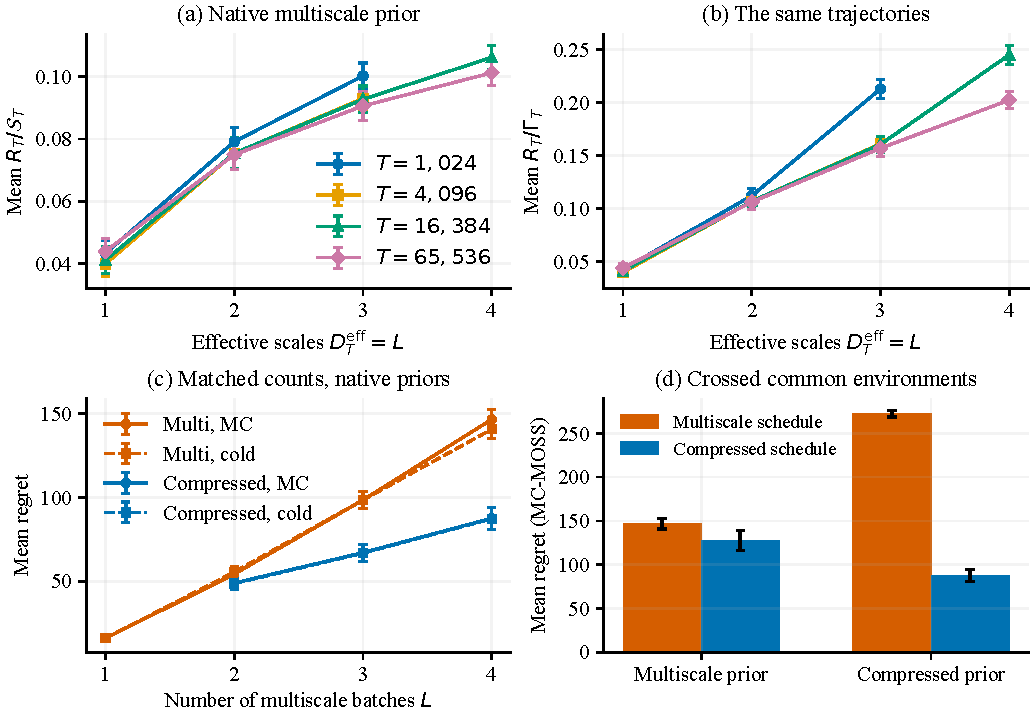
\includegraphics[width=\textwidth]{figures_v2/fig_geometry_risk.pdf}
 \caption{Bandit risk on a compatible finite product prior. Panels (a) and (b) use MC-MOSS and the native multiscale prior with gap multiplier four. Panel (c) compares each schedule under its native prior at $T=65536$; paired schedules have the same final count. Panel (d) fixes $T=65536$, $L=4$, and the sampled mean vector while changing its arrival schedule. Bars are $1.96$ Monte Carlo standard errors over 128 independent replications.}
 \label{fig:geometry-risk}
\end{figure}
